\documentclass[12pt]{scrartcl}

\usepackage{amsmath,amssymb}
\usepackage{fullpage}
\usepackage{enumitem}
\usepackage{hyperref}
\usepackage{graphicx}
\usepackage{tikz}
\usepackage{pgfplots}
\usepackage{float}
\usepackage{tabularx}
\usepackage{titlesec}

\pgfplotsset{compat=1.18}
\usetikzlibrary{trees,positioning,shapes,arrows}
\usepgfplotslibrary{statistics} 
\setlength{\parindent}{0pt}

\tikzset{
  basic/.style  = {draw, text width=2cm, drop shadow, font=\sffamily, rectangle},
  root/.style   = {basic, rounded corners=2pt, thin, align=center, fill=white},
  level-2/.style = {basic, rounded corners=6pt, thin,align=center, fill=white, text width=3cm},
  level-3/.style = {basic, thin, align=center, fill=white, text width=1.8cm}
}

\titleformat{\section}  % which section command to format
{\fontsize{12}{14}\bfseries} % format for whole line
{\thesection} % how to show number
{1em} % space between number and text
{} % formatting for just the text
[] % formatting for after the text

\titleformat{\subsection}  % which section command to format
{\fontsize{12}{14}\bfseries} % format for whole line
{\thesubsection} % how to show number
{1em} % space between number and text
{} % formatting for just the text
[] % formatting for after the text

\begin{document}

\begin{center}
	\hrule
	\vspace{0.4cm}
	{\textbf{\large Lecture 02: Probability Theory}}\\ [0.2cm]
	INF1004 Mathematics II

\end{center}

\textbf{Name:} Timothy Chia \hspace{\fill} \textbf{Date:} 12/01/2025 \\

\hrule

\section{Types of Probability}
Probability is defined as a number in the range $[0,1]$ that is assigned to an event associated with a random experiment. There are two interpretations of probability theory that guide how such values are assigned:

\subsection{Classical Probability}
In classical probability, all outcomes in the sample space are assumed to be equally likely.\\
The probability of a random event $A$ occuring is given as $$P(A)=\frac{\text{Number of different outcomes in A}}{\text{Total number of possible outcomes}}$$
\textbf{\textit{Note:}} This definition is not very practical for everyday life because it assumes the outcomes are equally likely.

\subsection{Empirical Probability}
In empirical probability theory, the probability of an event $A$ occurring  approximated by the relative frequency of its occurrence over a large number of trials such that $$P(A)=\frac{\text{Number of times an outcome occurs}}{\text{Total number of observations}}$$
This interpretation relies on collecting data over the years or existing historical data to propose such relative frequencies.

\subsection{Definitions}
\begin{itemize}
	\item We define a sample space $S$ as the set of all possible outcomes of a random phenomenon.
	\item An event $A$ is defined as the set of outcomes under investigation.
	\item By definition of probability, the following statements must hold to be valid: $$0 \leq P(A) \leq 1,\ P(S)=1$$
	\item If $A_1, A_2, \ldots$ are mutually exclusive events, then $$P\!\left(\bigcup_{i} A_i\right) = \sum_{i} P(A_i)$$.
\end{itemize}

%------------------------------------------------------------
\newpage
\section{Complementary Events}
The complement of an event $A$ denoted $P(A^c)$ and is given by $$P(A^c) = P(S) - P(A)$$

Conceptually, the complement of an event can be thought of as the probability that it does not occur. Visually, this can be represented as the area in a venn diagram that is not in $A$.

\begin{center}
	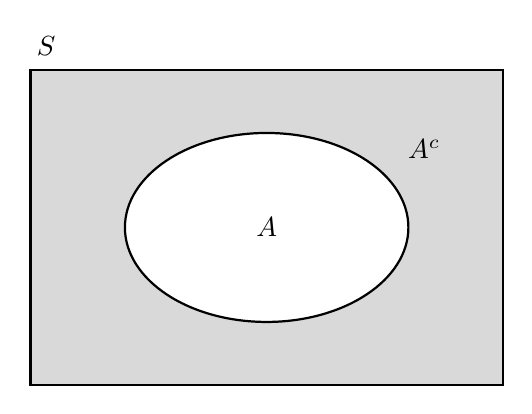
\begin{tikzpicture}
		% Sample space S
		\draw[thick, fill=gray!30] (0,0) rectangle (6,4);
		\node at (0.2,4.3) {$S$};

		% Event A
		\draw[thick, fill=white!30] (3,2) ellipse (1.8cm and 1.2cm);
		\node at (3,2) {$A$};

		% Complement label
		\node at (5,3) {$A^{c}$};
	\end{tikzpicture}
\end{center}

\section{Intersection of Events}
Given two events $A$ and $B$, the probability of their intersection denoted $$P(A \cap B)$$ is the probability that both events occur. In a venn diagram, it is the area where both events overlap.

\begin{center}
	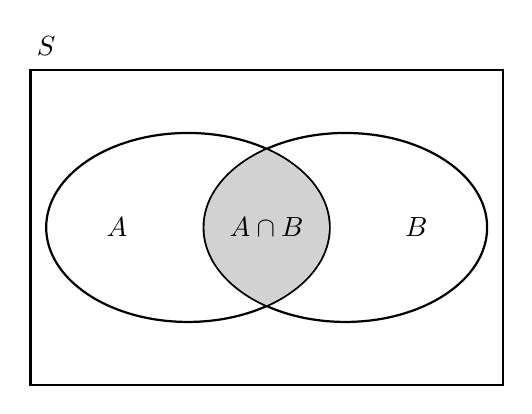
\begin{tikzpicture}
		% Sample space
		\draw[thick] (0,0) rectangle (6,4);
		\node at (0.2,4.3) {$S$};

		% Circles/ellipses outlines (unfilled)
		\draw[thick] (2,2) ellipse (1.8cm and 1.2cm);
		\draw[thick] (4,2) ellipse (1.8cm and 1.2cm);


		% Shade intersection only (clip trick)
		\begin{scope}
			\clip (2,2) ellipse (1.79cm and 1.19cm);
			\fill[gray!35] (4,2) ellipse (1.79cm and 1.19cm);
		\end{scope}

		% Labels
		\node at (1.1,2) {$A$};
		\node at (4.9,2) {$B$};
		\node at (3,2) {$A \cap B$};
	\end{tikzpicture}
\end{center}

If two events $A$ and $B$ are mutually exclusive, then $P(A \cap B) = 0$ because both events never overlap.

%------------------------------------------------------------
\newpage
\section{Union of Events}

Given two events $A$ and $B$, the \emph{union} of these events, denoted $A \cup B$, is the event that \emph{at least one} of the events occurs. That is, $A \cup B$ occurs if event $A$ occurs, or event $B$ occurs, or both occur.\\[0.2cm]
In terms of probability, $P(A \cup B)$ represents the probability that at least one of the two events occurs. Visually, in a Venn diagram, the union corresponds to the total area covered by both events $A$ and $B$.

\begin{center}
	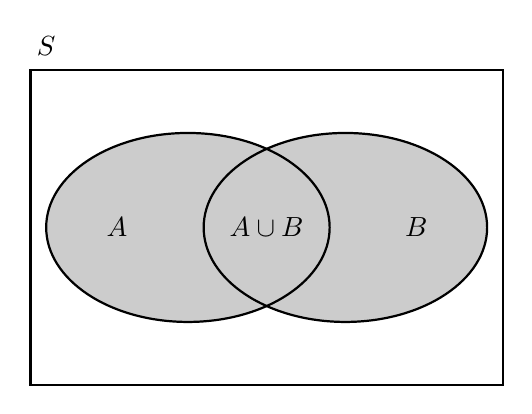
\begin{tikzpicture}[scale=1]
		% Sample space
		\draw[thick] (0,0) rectangle (6,4);
		\node at (0.2,4.3) {$S$};

		% Filled union region
		\fill[gray!40] (2,2) ellipse (1.8cm and 1.2cm);
		\fill[gray!40] (4,2) ellipse (1.8cm and 1.2cm);

		% Event outlines
		\draw[thick] (2,2) ellipse (1.8cm and 1.2cm);
		\draw[thick] (4,2) ellipse (1.8cm and 1.2cm);

		% Labels
		\node at (1.1,2) {$A$};
		\node at (4.9,2) {$B$};
		\node at (3,2) {$A \cup B$};
	\end{tikzpicture}
\end{center}

In general, the probability of the union of two events is given by
\[
	P(A \cup B) = P(A) + P(B) - P(A \cap B).
\]

This formula accounts for the fact that the overlapping region $A \cap B$ is included in both $P(A)$ and $P(B)$, and therefore must be subtracted once to avoid double counting.

\medskip

\subsection{Mutually Exclusive Events}
If events $A$ and $B$ are \emph{mutually exclusive}, then they cannot occur at the same time. In this case,
\[
	P(A \cap B) = 0,
\]
and the formula simplifies to
\[
	P(A \cup B) = P(A) + P(B).
\]

%------------------------------------------------------------
\newpage
\section{Conditional Probabilities}
In practice, it happens naturally that probability of an event $A$ can be changed if additional information is available, which leads to the discovery/creation of \emph{conditional probability}.

\subsection{Definition}
The conditional probability of event $A$ given that event $B$ has occurred, denoted $P(A \mid B)$, is defined (for $P(B) > 0$) as $$P(A \mid B) = \frac{P(A \cap B)}{P(B)}.$$

\begin{center}
	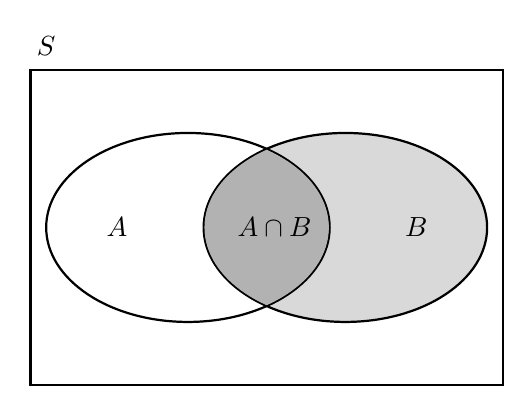
\begin{tikzpicture}[scale=1]

		% Sample space
		\draw[thick] (0,0) rectangle (6,4);
		\node at (0.2,4.3) {$S$};

		% Event B (conditioning event)
		\fill[gray!30] (4,2) ellipse (1.8cm and 1.2cm);
		\draw[thick] (4,2) ellipse (1.8cm and 1.2cm);

		% Event A
		\draw[thick] (2,2) ellipse (1.8cm and 1.2cm);

		% Intersection A ∩ B
		\begin{scope}
			\clip (4,2) ellipse (1.79cm and 1.19cm);
			\fill[gray!60] (2,2) ellipse (1.79cm and 1.19cm);
		\end{scope}

		% Labels
		\node at (1.1,2) {$A$};
		\node at (4.9,2) {$B$};
		\node at (3.1,2) {$A \cap B$};

	\end{tikzpicture}
\end{center}


\textbf{\textit{Note:}} Conditional probability is \emph{not symmetric}. In general,
\[
	P(A \mid B) \neq P(B \mid A),
\]
because the events $A$ and $B$ may have different probabilities and provide different information when conditioned upon.

\medskip

Additionally, when working with conditional probability $P(A \mid B)$, the sample space is no longer the original sample space $S$. Instead, the sample space is restricted to event $B$. All probabilities are therefore measured \emph{relative to $B$}.


%------------------------------------------------------------
% \newpage
\section{Multiplicative Rule of Probability}

The definition of conditional probability provides a way to compute the intersection of events $A$ and $B$. Since,
\begin{align*}
	P(A \mid B) & = \frac{P(A \cap B)}{P(B)}, \\
	P(B \mid A) & = \frac{P(A \cap B)}{P(A)}.
\end{align*}

We have that,
\begin{align*}
	P(A \cap B) & = P(A \mid B) \cdot P(B), \\
	P(A \cap B) & = P(A \mid B) \cdot P(A).
\end{align*}

%------------------------------------------------------------
\newpage
% \section{Independent and Mutually Exclusive Events}
%
% Events may be related in different ways depending on how the occurrence of one affects another.
% Two important relationships are \emph{independence} and \emph{mutual exclusivity}.
% These concepts are fundamentally different and should not be confused.
%
% \medskip
%
% \textbf{Independent events} may occur together, but the occurrence of one does not affect the probability of the other.
%
% \begin{center}
% 	\begin{tikzpicture}[scale=1]
% 		% Sample space
% 		\draw[thick] (0,0) rectangle (6,4);
% 		\node at (0.2,4.3) {$S$};
%
% 		% Events
% 		\draw[thick] (2.5,2) ellipse (1.6cm and 1.1cm);
% 		\draw[thick] (3.5,2) ellipse (1.6cm and 1.1cm);
%
% 		% Labels
% 		\node at (2,2) {$A$};
% 		\node at (4,2) {$B$};
% 	\end{tikzpicture}
% \end{center}
%
% \medskip
%
% \textbf{Mutually exclusive events} cannot occur at the same time, so their intersection is empty.
%
% \begin{center}
% 	\begin{tikzpicture}[scale=1]
% 		% Sample space
% 		\draw[thick] (0,0) rectangle (6,4);
% 		\node at (0.2,4.3) {$S$};
%
% 		% Events
% 		\draw[thick] (2,2) ellipse (1.4cm and 1.1cm);
% 		\draw[thick] (4,2) ellipse (1.4cm and 1.1cm);
%
% 		% Labels
% 		\node at (2,2) {$A$};
% 		\node at (4,2) {$B$};
% 	\end{tikzpicture}
% \end{center}
%
% \subsection{Independent Events}
%
% Two events $A$ and $B$ are said to be \textbf{independent} if
% \[
% 	P(A \cap B) = P(A)\,P(B).
% \]
%
% Equivalently, provided the relevant probabilities are non-zero,
% \[
% 	P(A \mid B) = P(A)
% 	\quad \text{or} \quad
% 	P(B \mid A) = P(B).
% \]
%
% That is, the occurrence of one event does not affect the probability of the other. Using the definition of conditional probability,
% \[
% 	P(A \cap B) = P(A \mid B)\,P(B).
% \]
% If $A$ and $B$ are independent, then $P(A \mid B) = P(A)$, and hence
% \[
% 	P(A \cap B) = P(A)\,P(B).
% \]
%
% This result is known as the \textbf{multiplication rule for independent events}.
%
% \medskip
%
% More generally, if $A_1, A_2, \dots, A_n$ are mutually independent events, then the probability that all events occur is
% \[
% 	P\!\left( \bigcap_{i=1}^{n} A_i \right)
% 	= \prod_{i=1}^{n} P(A_i).
% \]

\newpage
\section{Independent and Mutually Exclusive Events}

Events may be related in different ways depending on how the occurrence of one affects another.
Two important relationships are \emph{independence} and \emph{mutual exclusivity}.
These concepts are fundamentally different and should not be confused.

\medskip

% --- Side-by-side diagrams (fixed) ---
\noindent
\begin{minipage}[t]{0.48\linewidth}
	\centering
	\textbf{Independent Events}

	\medskip

	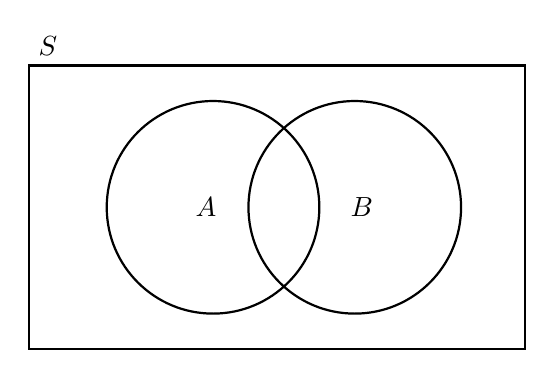
\begin{tikzpicture}[scale=0.9]
		% Sample space
		\draw[thick] (0,0) rectangle (7,4);
		\node[anchor=south west] at (0,4) {$S$};

		% Events (overlap is allowed)
		\draw[thick] (2.6,2) ellipse (1.5cm and 1.5cm);
		\draw[thick] (4.6,2) ellipse (1.5cm and 1.5cm);

		% Labels
		\node at (2.5,2) {$A$};
		\node at (4.7,2) {$B$};
	\end{tikzpicture}

	\medskip
	Both events may occur, but the occurrence of one does not affect the probability of the other.
\end{minipage}
\hfill
\begin{minipage}[t]{0.48\linewidth}
	\centering
	\textbf{Mutually Exclusive Events}

	\medskip

	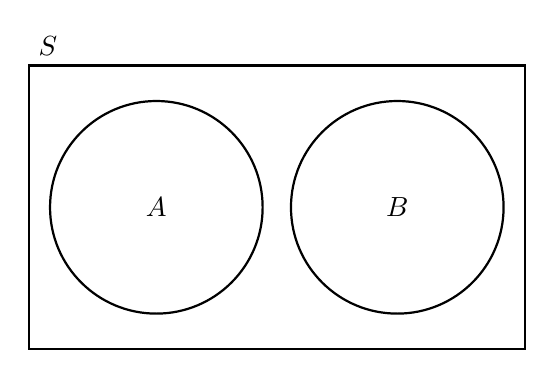
\begin{tikzpicture}[scale=0.9]
		% Sample space
		\draw[thick] (0,0) rectangle (7,4);
		\node[anchor=south west] at (0,4) {$S$};

		% Events (NO overlap)
		\draw[thick] (1.8,2) ellipse (1.5cm and 1.5cm);
		\draw[thick] (5.2,2) ellipse (1.5cm and 1.5cm);

		% Labels
		\node at (1.8,2) {$A$};
		\node at (5.2,2) {$B$};
	\end{tikzpicture}

	\medskip
	Events cannot occur at the same time, so \(A \cap B = \varnothing\). (e.g. If A happens, B cannot—so learning A occurred rules B out.)
\end{minipage}

\medskip

\textbf{\textit{Note:}} Independent events may overlap, whereas mutually exclusive events never do.

\subsection{Independent Events}

Two events $A$ and $B$ are said to be \textbf{independent} if
\[
	P(A \cap B) = P(A)\,P(B).
\]

Equivalently, provided the relevant probabilities are non-zero,
\[
	P(A \mid B) = P(A)
	\quad \text{or} \quad
	P(B \mid A) = P(B).
\]

That is, the occurrence of one event does not affect the probability of the other.
Using the definition of conditional probability,
\[
	P(A \cap B) = P(A \mid B)\,P(B).
\]
If $A$ and $B$ are independent, then $P(A \mid B) = P(A)$, and hence
\[
	P(A \cap B) = P(A)\,P(B).
\]

This result is known as the \textbf{multiplication rule for independent events}.

\medskip

More generally, if $A_1, A_2, \dots, A_n$ are mutually independent events, then the probability that all events occur is
\[
	P\!\left( \bigcap_{i=1}^{n} A_i \right)
	= \prod_{i=1}^{n} P(A_i).
\]

%------------------------------------------------------------
\newpage
% \section{Law of Total Probability}
%
% The Law of Total Probability is a rule that lets you calculate the probability of an event by breaking it down into several mutually exclusive cases that together cover all possibilities.
%
% \begin{center}
% 	\begin{tikzpicture}[scale=1]
%
% 		% Sample space
% 		\draw[thick] (0,0) rectangle (8,4);
% 		\node at (0.3,4.3) {$S$};
%
% 		\node at (1.35,3.6) {$S_1$};
% 		\node at (4,3.6) {$S_2$};
% 		\node at (6.7,3.6) {$S_3$};
%
% 		% Event A (ellipse)
% 		\fill[gray!40] (4,1.8) ellipse (2.9cm and 1.4cm);
% 		\draw[thick] (4,1.8) ellipse (2.9cm and 1.4cm);
%
% 		% % Labels for intersections
% 		\node at (2.1,1.8) {$A \cap S_1$};
% 		\node at (4,1.8) {$A \cap S_2$};
% 		\node at (5.9,1.8) {$A \cap S_3$};
%
% 		% Partition lines (S1, S2, S3)
% 		\draw[dashed] (2.9,0) -- (2.9,4);
% 		\draw[dashed] (5.1,0) -- (5.1,4);
%
% 	\end{tikzpicture}
% \end{center}

\section{Law of Total Probability}

The \textbf{Law of Total Probability} allows us to compute the probability of an event by decomposing the sample space into several mutually exclusive and exhaustive cases.

\subsection{Definition}

Suppose $S_1, S_2, \dots, S_n$ form a \textbf{partition} of the sample space $S$, meaning:
\begin{itemize}
	\item $S_i \cap S_j = \varnothing$ for $i \neq j$ (mutually exclusive),
	\item $\displaystyle \bigcup_{i=1}^{n} S_i = S$ (exhaustive),
	\item $P(S_i) > 0$ for all $i$.
\end{itemize}

Then for any event $A \subseteq S$, we may write $A$ as the union of its intersections with each $S_i$:
\[
	A = (A \cap S_1) \cup (A \cap S_2) \cup \cdots \cup (A \cap S_n).
\]

Since these intersections are mutually exclusive, their probabilities add, giving
\[
	P(A) = P(A \cap S_1) + P(A \cap S_2) + \cdots + P(A \cap S_n).
\]

This concept can be visualised with the following Venn diagram.

\begin{center}
	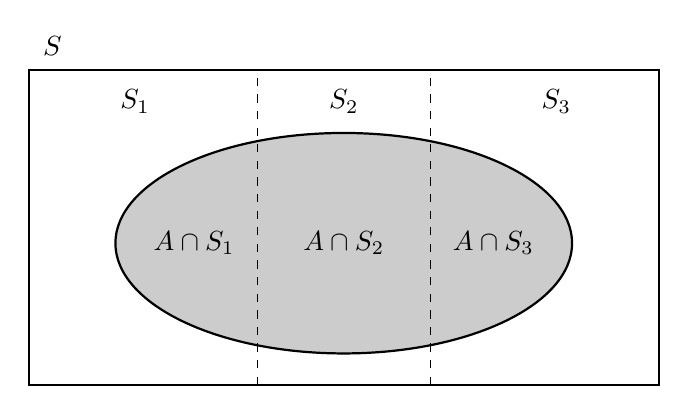
\begin{tikzpicture}[scale=1]

		% Sample space
		\draw[thick] (0,0) rectangle (8,4);
		\node at (0.3,4.3) {$S$};

		\node at (1.35,3.6) {$S_1$};
		\node at (4,3.6) {$S_2$};
		\node at (6.7,3.6) {$S_3$};

		% Event A
		\fill[gray!40] (4,1.8) ellipse (2.9cm and 1.4cm);
		\draw[thick] (4,1.8) ellipse (2.9cm and 1.4cm);

		% Intersection labels
		\node at (2.1,1.8) {$A \cap S_1$};
		\node at (4,1.8) {$A \cap S_2$};
		\node at (5.9,1.8) {$A \cap S_3$};

		% Partition lines
		\draw[dashed] (2.9,0) -- (2.9,4);
		\draw[dashed] (5.1,0) -- (5.1,4);

	\end{tikzpicture}
\end{center}

Using the definition of conditional probability,
\[
	P(A \cap S_i) = P(A \mid S_i)\,P(S_i).
\]

Substituting this into the previous expression yields the \textbf{Law of Total Probability}:
\[
	P(A) = \sum_{i=1}^{n} P(A \mid S_i)\,P(S_i).
\]


%------------------------------------------------------------
\newpage
\section{Bayes' Theorem}

Bayes’ Theorem provides a way to reverse conditional probabilities. In particular, it allows us to compute $P(B \mid A)$ in terms of $P(A \mid B)$, together with prior information about $B$. From the definition of conditional probability, we have
\[
	P(A \mid B) = \frac{P(A \cap B)}{P(B)}
	\quad \text{and} \quad
	P(B \mid A) = \frac{P(A \cap B)}{P(A)}.
\]

Rearranging the first expression gives
\[
	P(A \cap B) = P(A \mid B)\,P(B).
\]

Substituting this into the second expression yields \textbf{Bayes’ Theorem}:
\[
	P(B \mid A) = \frac{P(A \mid B)\,P(B)}{P(A)}.
\]

\medskip

In practice, the probability $P(A)$ in the denominator is often unknown directly. It is commonly computed using the \textbf{Law of Total Probability}.

\medskip

Suppose $B$ and $B^{c}$ form a partition of the sample space, meaning they are mutually exclusive and exhaustive. Then
\[
	P(A) = P(A \mid B)\,P(B) + P(A \mid B^{c})\,P(B^{c}).
\]

Substituting this into Bayes’ Theorem gives the expanded form:
\[
	P(B \mid A)
	=
	\frac{P(A \mid B)\,P(B)}
	{P(A \mid B)\,P(B) + P(A \mid B^{c})\,P(B^{c})}.
\]

This formulation highlights how Bayes’ Theorem updates the probability of an event using new information, weighted by prior probabilities.

\end{document}
